\documentclass[11pt,a4paper]{article}
%\documentclass[11pt,a4paper,draft]{book}

%%% Packages
\usepackage{Styles/reportstyle}
%\usepackage{Styles/unipitesi}
\usepackage{Styles/commands}

\usepackage{amsfonts}
\lstset{language=Python}
%%%
\title{Immagini animate e Tensor Train.\\Compressione e suoi effetti su dati ``visibili''.}
\author{Tommaso Bianucci}
%%%
\begin{document}
\maketitle

\begin{abstract}
  La \emph{Tensor Train Decomposition} (\emph{TT}), è un formato di rappresentazione di tensori di recente sviluppo che ha come principale obiettivo quello di fornire una buona approssimazione del tensore iniziale utilizzando un numero ridotto di \emph{parametri}, analogamente a quanto la \emph{SVD} permette di fare con le matrici.

  %% In particolare, questo metodo di rappresentazione \emph{rompe} la diendenza esponenziale dal numero di dimensioni, rendendo finalmente possibili applicazioni con alta dimensionalità.
  %% Per questo possiamo riferirci alla TT come strumento di \emph{compressione} di dati, in quanto permette di manipolare dati dalla elevata dimensionalità con un'impronta in memoria relativamente ridotta.

  La qualità della rappresentazione è stata definita e dimostrata da risultati teorici, ma cosa questa comporti a livello qualitativo sui dati in ingresso resta difficile da immaginare, complicato inoltre dalla intrinseca difficoltà di rappresentazione di dati a più di 3 dimensioni.

  La compressione di immagini è un classico esempio che permette apprezzare immediatamente il risultato della SVD, così abbiamo utilizzato un approccio analogo con la TT, comprimendo brevi animazioni.
  Le immagini animate costituiscono infatti un facile esempio di dato in 4 dimensioni: larghezza, altezza, colore e numero di frame.
  Abbiamo quindi compresso le animazioni in formato TT, misurato il \emph{rapporto di compressione} e ricostruito le animazioni approssimate per un facile confronto visivo con l'originale. \todo{Rivedi, anche alla luce di quanto riutilizzato sotto in Obiettivi}
\end{abstract}

%\listoftodos
\tableofcontents

%%% WRITE TEXT HERE
\section{Obiettivi}
La \emph{Tensor Train Decomposition}, o più brevemente \emph{TT}, è un formato di rappresentazione di tensori\footnote{Con tensore intendiamo genericamente un array multidimensionale.} di recente sviluppo che ha come principale obiettivo quello di fornire una buona approssimazione del tensore iniziale utilizzando un numero ridotto di \emph{parametri}, analogamente a quanto la \emph{SVD} permette di fare con le matrici.
In particolare, questo metodo di rappresentazione \emph{rompe} la dipendenza esponenziale dal numero di dimensioni, rendendo finalmente possibili applicazioni con alta dimensionalità.
Per questo possiamo riferirci alla TT come strumento di \emph{compressione} di dati, in quanto permette di manipolare dati dalla elevata dimensionalità con un'impronta in memoria relativamente ridotta.

  La qualità della rappresentazione è stata definita e dimostrata da risultati teorici, ma cosa questa comporti a livello qualitativo sui dati in ingresso resta difficile da immaginare, complicato inoltre dalla intrinseca difficoltà di rappresentazione di dati a più di 3 dimensioni.

  La compressione di immagini è un classico esempio che permette, letteralmente, di visualizzare il risultato della SVD, apprezzandone intuitivamente le caratteristiche principali. Così abbiamo pensato di seguire un approccio analogo con la TT: comprimere immagini, per poterne visualizzare immediatamente il risultato.

\section{Approccio}
Un tensore rappresentato in formato TT consta di un insieme di tensori 3-dimensionali i cui elementi, opportunamente moltiplicati tra di loro, restituiscono tutti gli elementi, entro un certo grado di approssimazione, del tensore di partenza.
Questo lascia immediatamente intuire come i vantaggi del formato TT siano tanto maggiori quanto maggiore è la dimensionalità del tensore originario e anche come i benefici su tensori 3-dimensionali siano esigui se non assenti da un punto di vista di spazio utilizzato e sicuramente vanificati dalla complessità e dal tempo computazionale aggiuntivi che la rappresentazione in formato TT richiedono.

Con questa premessa abbiamo cercato una tipologia di dati che avesse un numero di dimensioni maggiore di 3 e che fosse facilmente visualizzabile. La scelta è caduta sulle immagini animate.

Le sequenze animate si prestano naturalmente ad essere rappresentate in 4 dimensioni, infatti
\begin{itemize}
\item queste sono certamente un insieme ordinato di immagini (\emph{frames}),
\item ogni frame è composto da una matrice di \emph{pixel},
\item ogni pixel può emettere i 3 colori primari (RGB\footnote{\emph{RGB} = red-green-blue (rosso-verde-blu), i tre colori primari per la sintesi sottrattiva.}), ognuno caratterizzato da un proprio valore di luminosità.
\end{itemize}
In 4 dimensioni si strutturano quindi i dati di una sequenza animata: numero di frame per identificare la posizione temporale, larghezza e altezza per identificare la posizione spaziale del pixel, colore. Gli elementi del tensore assumeranno quindi valori tra $0$ e $255$ e rappresenteranno la luminosità di un dato colore per un certo pixel all'interno di uno specifico frame.

\section{Implementazione, problemi e compromessi}
Per l'implementazione abbiamo utilizzato il seguente approccio:
\begin{itemize}
\item estrarre i singoli frame dalle animazioni GIF in ingresso e convertirli in formato PPM utilizzando il comando \rawcode{convert} dalla suite \href{http://www.imagemagick.org/}{Imagemagick},
\item leggere i frame per popolare gli elementi di un tensore di dimensioni adeguate,
\item approssimare iterativamente il tensore utilizzando l'algoritmo \emph{tt-cross} dalla libreria \href{https://github.com/oseledets/ttpy}{\emph{ttpy}} di Ivan Oseledets,
\item estrarre i valori per ogni frame e scriverli in un nuovo file PPM,
\item infine ricomporre i file PPM risultanti in una nuova animazione GIF.
\end{itemize}

\subsection{Linguaggi utilizzati}
Le operazioni di estrazione, conversione a PPM e ricomposizione dei frame dal o verso il formato GIF sono state organizzate semplicemente sotto forma di brevi script in Bash. Invece la parte saliente di lettura dei frame, approssimazione in formato TT e riscrittura dei nuovi frame è stata implementata in linguaggio Python.

La scelta di utilizzare Python è risultata dal considerare che
\begin{itemize}
\item Python è un linguaggio flessibile e agevole, tipizzato dinamicamente e che non richiede una gestione manuale dell'allocazione di memoria, rendendo la prototipazione e cambiamenti anche radicali molto agevoli e veloci,
\item è disponibile, per Python, il modulo \emph{ttpy}, che implementa la rappresentazione e i vari algoritmi per la compressione e la manipolazione di tensori in formato TT,
\item Python è un linguaggio notoriamente poco performante, ma il modulo \emph{ttpy} implementa tutte le operazioni computazionalmente intense e critiche in linguaggio Fortran, avvalendosi dove possibile di subroutine da LaPack/BLAS.
\end{itemize}
In questo modo è stato possibile mantenere i vantaggi di un linguaggio come Python, pur mantenedo tutte le fasi computazionalmente più costose in opportune subroutine Fortran e quindi non intaccando le prestazioni complessive dell'intero processo.

\subsection{TT-cross e criteri d'arresto}
\paragraph{TT-cross.}
L'algoritmo di TT-cross è basato sull'approssimazione iterativa di un tensore tramite l'utilizzo, ad ogni passo, di alcuni specifici elementi.
Questo permette la costruzione di un un'approssimazione TT anche in assenza del tensore completo di partenza. Infatti è sufficiente avere a disposizione una funzione che permetta di calcolare, date le coordinate di un elemento, il suo valore.

Noi costruiamo esplicitamente l'intero tensore di partenza, popolandolo con i valori che vengono letti dai file che contengono i vari frame: questo non ci danneggia, visto che lo spazio richiesto in questa operazione è nel nostro caso davvero modesto, e ci avvantaggia in termini di tempo. Abbiamo comunque definito una funzione che ci restituisce l'elemento del tensore date le coordinate, in modo da poterla utilizzare nell'algoritmo TT-cross.

\paragraph{Misurare l'errore.}
Per decidere quando arrestare l'iterazione, abbiamo bisogno di definire una misura di errore.

Per il nostro scopo di comprimere animazioni, abbiamo deciso di affidarci ad un metodo molto semplice ma che ha dimostrato di dare buoni risultati: vengono campionati casualmente l'1\% degli elementi del tensore e viene quindi calcolata la distanza dal corrispondente valore nel tensore originario; se l'elemento è all'interno di un raggio di 5 unità di luminosità dal corrispondente valore del tensore originario, viene considerato valido, altrimenti non valido.
La percentuale di valori validi sul totale campionato è quindi considerata un parametro indice della verosimiglianza dell'animazione compressa rispetto all'originale.

La scelta è caduta su questo criterio, a dire il vero piuttosto \emph{artigianale}, dopo aver osservato che l'errore relativo, così come misurato internamente durante l'algoritmo di TT-cross\todo{Controlla bene come è calcolato l'errore internamente in TT-cross}, convergeva troppo lentamente e a valori non generalizzabili ai vari esempi di input provati, sebbene i risultati in uscita fossero sufficientemente accurati da un punto di vista visivo.

\paragraph{Criteri d'arresto.}
Come menzionato nel precedente paragrafo, per questa applicazione ci siamo affidati ad un criterio d'arresto \emph{ad-hoc}: quando una percentuale sufficientemente alta di elementi presenta un errore al di sotto di un certo valore, l'approssimazione viene fermata.

Come intuibile, questo criterio presenta il grande difetto di non tenere in considerazione quanto errore presentino gli altri elementi, quelli che non hanno superato il test.
D'altra parte però questo criterio ci permette di terminare l'approssimazione non appena una parte sufficiente dell'animazione bene approssima l'originale.

Questa scelta, del tutto arbitraria e volta a contenere i tempi di convergenza ed il numero di parametri necessario, lascia passare nelle immagini finali alcuni artefatti degni di nota. Ad esempio può portare alcune parti dell'immagine ad avere valori di colore/luminosità molto instabili nel tempo, mentre altre parti risultano ben definite. Oppure si possono avere parti dell'immagine che ricompaiono come \emph{fantasmi} in frame \todo{Controlla se si può dire aliasing nella footnote.} multipli.\footnote{A questo proposito è bene ricordare come il \emph{tempo} altro non sia che una dimensione del tensore al pari delle altre e quindi presenti dei fenomani di aliasing al pari delle dimensioni \emph{spaziali}. Quindi medesimi valori possono propagrsi all'interno dello stesso frame, sotto forma di \emph{bande} orizzontali o verticali, ma anche attraverso più frame, sotto forma di zone di immagine \emph{fantasma}.}

\subsection{Ottimizzazione delle performance}
In una prima implementazione, \todo{Qui parla di come read/write dei frame rischaissero di essere le fasi più costose in termini di tempo e di come questo sia stato risolto (soprattutto per il write che contiene gazillioni di moltiplicazioni tra matrici).} abbiamo osservato come la maggior frazione del tempo veniva spesa nella fase di scrittura dei frame invece che in quella di TT-cross.
Questo succedeva a causa del seguente codice: 

\begin{lstlisting}
  for row in range(height):
      rowput = [ str(pixelRound(x, maxval=depth)) + " " for x in 
                      frame[:,:,row]
                      .full()
                      .reshape(3*width, order='F') ]
      f.writelines(rowput)
      f.write('\n')
\end{lstlisting}

Questa confezionava una riga del frame corrente prendendo, in formato TT, la matrice $3 \times width$ corrispondente alla riga, calcolandone tutti gli elementi (con il metodo \rawcode{full()}, e facendo quindi un reshape per ottenere la concatenazione dei valori di colore per ogni pixel.

Ci sono principalmente due motivi per cui questo era inefficiente.
Il primo è che il metodo \rawcode{full()} è computazionalmente molto costoso, in quanto implica $\prod_{j=1}^d n_j (d-1)$ moltiplicazioni di matrici per un tensore $n_1 \times \ldots \times n_d$. Nel nostro caso, questa operazione comportava, per ogni riga, $2 \cdot 3 \cdot width$ moltiplicazioni di matrici, per un totale di $6 \cdot width \cdot height$ moltiplicazioni di matrici per frame, visto che l'operazione veniva eseguita in un ciclo indicizzato dal numero di riga. Il problema è che una buona parte di queste moltiplicazioni è ridondante: infatti quando si fissano tutti gli elementi di un tensore tranne uno, tutte le matrici da moltiplicare resteranno invariate tranne quella corrispondente alla dimensione su cui scorre quest'ultimo. Quindi, per ottenere tutti gli elementi di una data \emph{fibra} del tensore, ad esempio sulla dimensione $k$, dobbiamo calcolare $n_k (d-1)$ moltiplicazioni di matrici, quando le necessarie sarebbero soltanto $(d-2) + n_k$.

Il secondo motivo di inefficienza risiede nell'uso del metodo \rawcode{reshape()}: infatti \rawcode{full()} altro non fa se non calcolare tutti gli elementi del dato tensore in modo sequenziale, restituendoli in un array monodimensionale e applicando poi l'opportuno reshape per ottenere il tensore. Il problema è che, nel nostro codice, abbiamo bisogno di applicare un ulteriore \rawcode{reshape(3*width, order='F')}, di fatto rendendo il primo superfluo.

Abbiamo risolto il primo problema semplicemente calcolandoci tutti i valori di un intero frame con una sola chiamata di \rawcode{full}, invece che dovendone fare una per ogni riga. Infatti, con un opportuna manipolazione possiamo ottenere una lista di righe da poter scrivere nel file, senza dover iterare sulle righe come in precedenza. Questo risolve problema in quanto il metodo \rawcode{full()} è in grado di ottimizzare il numero di moltiplicazioni di matrici da eseguire.

Il secondo problema è invece stato risolto cambiando il metodo \rawcode{full()} nella libreria \emph{ttpy} in modo da poter accettare come argomento opzionale uno \emph{shape} specifico da passare alla chiamata di \rawcode{reshape()} che esegue internamente. Questo evita il bisogno di chiamare ogni volta un secondo \rawcode{reshape()} per ottenere il formato desiderato.

Il risultato è il seguente codice, che restituisce direttamente una lista di righe, che vengono successivamente scritte del file per il frame corrente:
\begin{lstlisting}
    frameput = [ ' '.join(vectorStrPixelRound(x)) for x in 
                    (depth*frame)
                    .full(shape=(3*width,height))
                    .transpose() ]
    for row in range(height):
        f.write(frameput[row])
        f.write('\n')
\end{lstlisting}

Queste piccole modifiche hanno ridotto il tempo dedicato alla scrittura dei frame su file dall'ordine di alcune ore all'ordine di pochi minuti.

%% \paragraph{Lettura frame.}
%% foobar ciao

%% \paragraph{Scrittura frame.}
%% foobar

%% \paragraph{Modifiche \emph{ad-hoc} del modulo ttpy.}
%% foobar

\section{Risultati}
Da un punto di vista di rapporto di compressione non abbiamo ottenuto risultati degni di nota e questo è in linea con le aspettative. Infatti il vantaggio del formato TT sta nel disaccopiare il numero di parametri necessari dalla dipendenza esponenziale dal numero di dimensioni e non ci aspettavamo di vedere risultati rilevanti con sole 4 dimensioni.

Da un punto di vista qualitativo, invece, abbiamo potuto rilevare soprattutto la presenza di artefatti quali l'uniformità lungo delle specifiche \emph{bande} lungo le fibre e improvvisi cambi di luminosità e colore \todo{Inserire immagini.}.

La fase di calcolo della compressione a mostrato una convergenza assai lenta, soprattutto se paragonata con la convergenza che l'algoritmo di TT-cross ha dimostrato in alcuni esempi di natura matematica, come ad esempio nel caso tensori popolati con i valori assunti da una funzione multidimensionale. \todo{magari vedi di metterci esempio del vsin.} In particolare, è stato impossibile stabilire valori di errore relativo in norma che potessero essere utilizzati in maniera affidabile e con una certa generalità. Al contrario, la semplice misura dell'errore da noi utilizzata si è rivelata nei fatti utile ad avere un'approssimazione in ogni caso accettabile.

%% \def\wid{0.5}
%% \begin{wrapfigure}{L}{\wid\textwidth}
%%   \def\scal{0.47}
%%   \centering
%%   \begin{subfigure}[b]{\wid\textwidth}
%%     \centering
%%     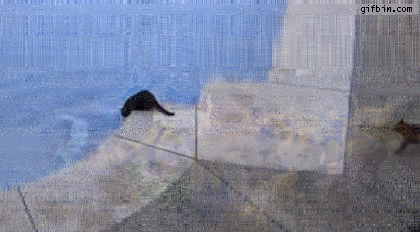
\includegraphics[keepaspectratio=true, scale=\scal]{Imgs/Cats/frame-10}
%%   \end{subfigure}
  
%%   \begin{subfigure}[b]{\wid\textwidth}
%%     \centering
%%     \includegraphics[keepaspectratio=true, scale=\scal]{Imgs/Cats/frame-11}
%%   \end{subfigure}
  
%%   \begin{subfigure}[b]{\wid\textwidth}
%%     \centering
%%     \includegraphics[keepaspectratio=true, scale=\scal]{Imgs/Cats/frame-12}
%%   \end{subfigure}
%%   \caption{Sequenza con elementi \emph{fantasma}.}\label{fig:cats_sequence_phantoms}
%% \end{wrapfigure}

%% \def\wid{0.5}
%% \begin{wrapfigure}{R}{\wid\textwidth}
%%   \def\scal{0.47}
%%   \centering
%%   \begin{subfigure}[b]{\wid\textwidth}
%%     \centering
%%     \includegraphics[keepaspectratio=true, scale=\scal]{Imgs/Cats/frame-105}
%%   \end{subfigure}
  
%%   \begin{subfigure}[b]{\wid\textwidth}
%%     \centering
%%     \includegraphics[keepaspectratio=true, scale=\scal]{Imgs/Cats/frame-111}
%%   \end{subfigure}
  
%%   \begin{subfigure}[b]{\wid\textwidth}
%%     \centering
%%     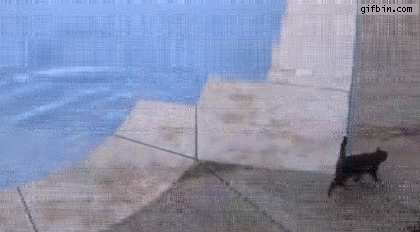
\includegraphics[keepaspectratio=true, scale=\scal]{Imgs/Cats/frame-113}
%%   \end{subfigure}
%%   \caption{Frame di provenienza.}\label{fig:cats_sequence_phantoms_comp}
%% \end{wrapfigure}

\begin{figure}
  \centering
  \def\wid{0.48}
  \def\scal{0.44}
  \begin{subfigure}[b]{\wid\textwidth}
    \begin{subfigure}[b]{\wid\textwidth}
      \centering
      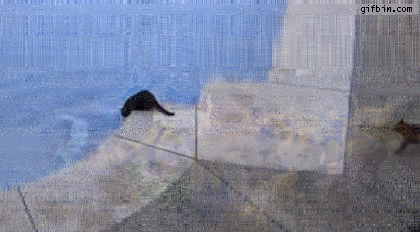
\includegraphics[keepaspectratio=true, scale=\scal]{Imgs/Cats/frame-10}
    \end{subfigure}
    
    \begin{subfigure}[b]{\wid\textwidth}
      \centering
      \includegraphics[keepaspectratio=true, scale=\scal]{Imgs/Cats/frame-11}
    \end{subfigure}
    
    \begin{subfigure}[b]{\wid\textwidth}
      \centering
      \includegraphics[keepaspectratio=true, scale=\scal]{Imgs/Cats/frame-12}
    \end{subfigure}
    \caption{Sequenza con elementi \emph{fantasma}.}\label{fig:cats_sequence_phantoms}
  \end{subfigure}
  ~
  \begin{subfigure}[b]{\wid\textwidth}
    \begin{subfigure}[b]{\wid\textwidth}
      \centering
      \includegraphics[keepaspectratio=true, scale=\scal]{Imgs/Cats/frame-105}
    \end{subfigure}
    
    \begin{subfigure}[b]{\wid\textwidth}
      \centering
      \includegraphics[keepaspectratio=true, scale=\scal]{Imgs/Cats/frame-111}
    \end{subfigure}
    
    \begin{subfigure}[b]{\wid\textwidth}
      \centering
      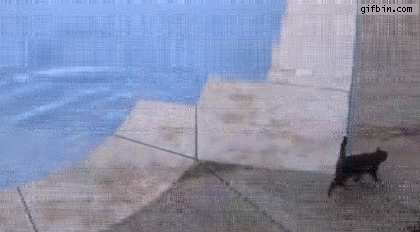
\includegraphics[keepaspectratio=true, scale=\scal]{Imgs/Cats/frame-113}
    \end{subfigure}
    \caption{Frame di provenienza.}\label{fig:cats_sequence_phantoms_comp}
  \end{subfigure}
  \caption{Elementi fantasma e rispettivi frame di provenienza.}
\end{figure}

Vediamo alcuni esempi di questi artefatti. La sequenza~\ref{fig:cats_sequence_phantoms} mostra tre frame consecutivi dall'animazione link\todo{Metti la gif intera su poisson e linkala qui!}: possiamo chiaramente vedere degli elementi \emph{fantasma} nella zona in basso a destra dell'immagine. Questi elementi provengono da frame successivi, visibili in \ref{fig:cats_sequence_phantoms_comp}. Sono ben visibili elementi di tutti e tre questi frame nella sequenza originale.

%\lipsum[2-5]

\def\widFrame{0.62}
\def\wid{0.6}
\def\scal{0.5}
\begin{wrapfigure}{R}{\widFrame\textwidth}
  \centering
  \begin{subfigure}[b]{\wid\textwidth}
    \centering
    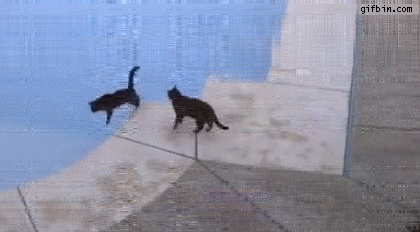
\includegraphics[keepaspectratio=true, scale=\scal]{Imgs/Cats/frame-62}
    \caption{Frange di rumore che si propagano verticalmente rispetto ai gatti.}\label{fig:cats_noise_vertical}
  \end{subfigure}
  
  \begin{subfigure}[b]{\wid\textwidth}
    \centering
    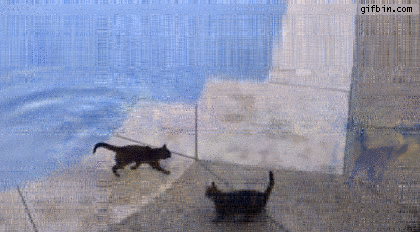
\includegraphics[keepaspectratio=true, scale=\scal]{Imgs/Cats/frame-94}
    \caption{Immagine fantasma sul lato destro dell'immagine}\label{fig:cats_noise_time}
  \end{subfigure}
  \caption{Propagazione di rumore e fantasmi lungo le fibre.}\label{fig:cats_noise}
\end{wrapfigure}

%%%% Tets
%% \def\widFrame{0.62}
%% \def\wid{0.6}
%% \def\scal{0.5}
%% \begin{wrapfigure}{R}{\widFrame\textwidth}
%%   \centering
%%   \begin{subfigure}[b]{\wid\textwidth}
%%     \centering
%%     \includegraphics[keepaspectratio=true, scale=\scal]{Imgs/MuhammadAli/frame-11}
%%     \caption{Frange di rumore che si propagano verticalmente rispetto ai gatti.}\label{fig:muhammadali_noise_vertical}
%%   \end{subfigure}
  
%%   \begin{subfigure}[b]{\wid\textwidth}
%%     \centering
%%     \includegraphics[keepaspectratio=true, scale=\scal]{Imgs/MuhammadAli/frame-12}
%%     \caption{Immagine fantasma sul lato destro dell'immagine}\label{fig:muhammadali_noise_time}
%%   \end{subfigure}
%%   \caption{Propagazione di rumore e fantasmi lungo le fibre.}\label{fig:muhammadali_noise}
%% \end{wrapfigure}

%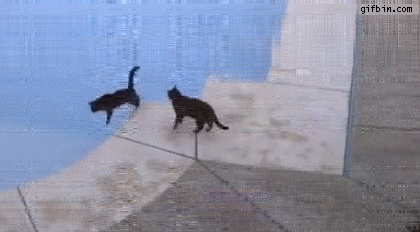
\includegraphics[keepaspectratio=true, scale=0.7]{Imgs/Cats/frame-62}
%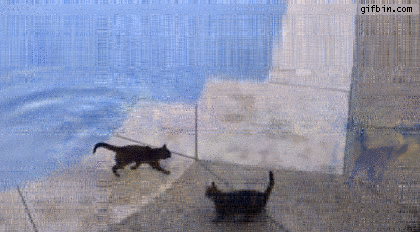
\includegraphics[keepaspectratio=true, scale=0.7]{Imgs/Cats/frame-94}

\section{Conclusioni}
Abbiamo raggiunto il nostro scopo di \emph{visualizzare} gli effetti dell'approssimazione tramite TT. Certamente la qualità dell'immagine, la presenza di vistosi artefatti e lo scarso livello di compressione ci fanno chiaramente capire come la compressione di filmati non sia il campo di applicazione di elezione del formato TT.
Dobbiamo però ricordare come il basso numero di dimensioni (4) e il vincolo di dover rappresentare valori in $[0,255]\subset\NN$ limitino l'efficacia dell'utilizzo del formato TT in questa applicazione.

%%%
\end{document}
